\chapter{Signals}

\begin{definition}[Signal]
   A signal is a real function of time
\end{definition}
\begin{itemize}
   \item Time-continuous and amplitude-continuous
   \item Time-continuous and quantized
   \item Time-discrete and amplitude-continuous
   \item Time-discrete and quantized
\end{itemize}


\section{Signal types}
\begin{paracol}{2}
   
   \colfill
   \begin{definition}[Continuous-time signal]
      A signal is continuous-time (also known as analog signals) if it is defined for all real numbers.
      The domain thus $\mathcal{D}$ is the set of real numbers $\mathbb{R}$\\
      If the codomain $\mathcal{C}$ is the set of real numbers $\mathbb{R}$:
      continuous amplitude signals.\\
      If the codomain $\mathcal{C}$ is a discrete set (e.g. $\mathbb{Z}$): discrete
      amplitude signals
      AKA quantized signals
   \end{definition}
   \colfill

   \switchcolumn

   \begin{figure}[htbp]
      \centering
      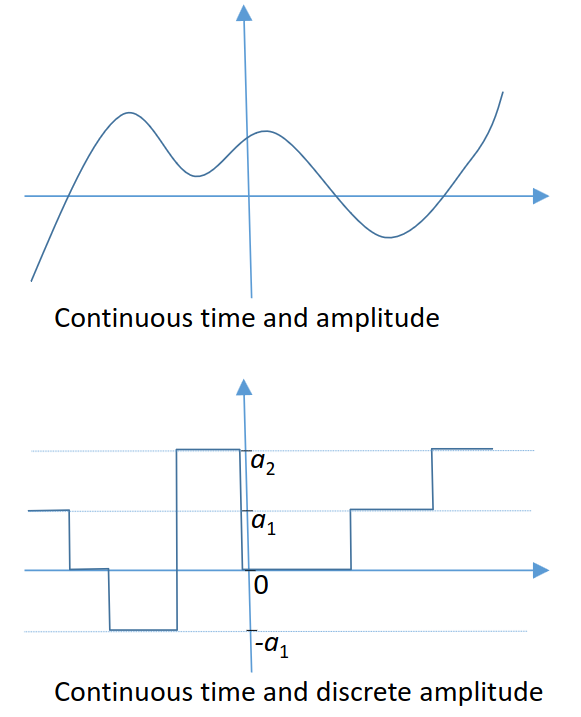
\includegraphics[width=0.4\columnwidth]{images/signals_continuous.png}
      \caption{Continous signals}
      \label{fig:signals_continuous}
   \end{figure}
\end{paracol}

\begin{paracol}{2}
   \colfill   
   \begin{definition}[Discrete-time signal]
      A signal is discrete-time if it is defined only at discrete times.\\
      The domain $\mathcal{D}$ is the set of integers $\mathbb{Z}_T$,
      where $\mathbb{Z}_T = \{nT, \forall n \in \mathbb{Z} \text{ and } T \in \mathbb{R}\}$.
      They are also called discrete signals.\\
      For example, $\mathbb{Z}_2 = \ldots, -4, -2, 0, 2, 4, \ldots$.
      
      A discrete signal is called digital when the codomain is a finite set of symbols.
      A digital signal is also called a symbolic sequence.
      A text is an example of a symbolic signal.
      
   \end{definition}
   \colfill

   \switchcolumn
   \begin{figure}[htbp]
      \centering
      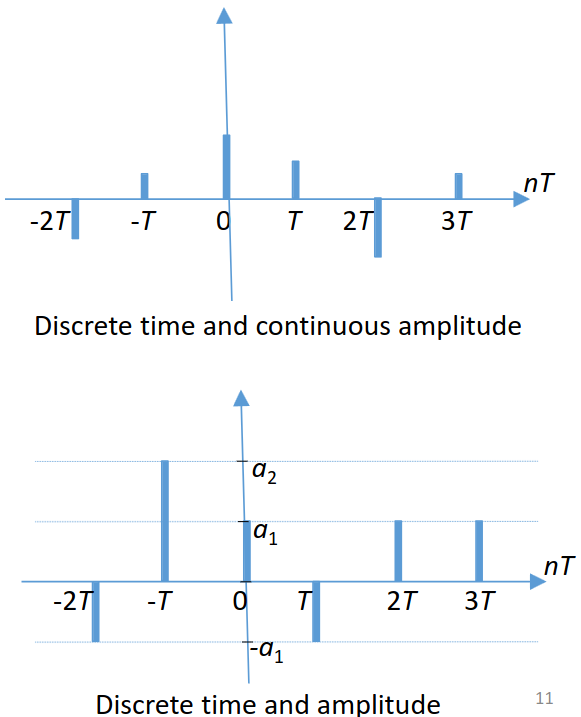
\includegraphics[width=0.4\columnwidth]{images/signals_discrete.png}
      \caption{Discrete signals}
      \label{fig:signals_discrete}
   \end{figure}
\end{paracol}


\begin{definition}[Digital signals]
   Consider the alphabet of the 26 symbols \texttt{A={a,b,c,\dots,x,y,z}}.
   A symbolic signal is any sequence of such symbols, e.g.:\\
   \texttt{ababfxje}\dots
   
   Consider now the alphabet of two symbols \texttt{B={0,1}}:
   \begin{itemize}
      \item We can represent any symbol in A with a sequence in B
      \item For example: \texttt{a $\cong$ 00000}, \texttt{b $\cong$ 00001}, etc.
      \item Hence, the digital signal \texttt{ababfxje} would become:\\
      \texttt{0000000001000000000100101101110100100100}
   \end{itemize}

   Assume a source that samples an analog signal with $f_c samples/second$.
   Each sample is represented (quantized) with $M bit/sample$.\\
   The source has a \textbf{throughput} of $f_c \cdot M bit/second$


\end{definition}

\section{Transmission of information}
Signals may have different nature,
depending on the channel, e.g. electromagnetic, sound, optical waves etc.
At the source a transducer converts a
message into a signal, which propagates
through a medium, while at the destination another transducer converts a signal into a message.
\note{For example, the antenna is a transducer for
electromagnetic signals}

\subsection{Disturbed}
\textbf{Distortion} refers to any change in a signal that alters the basic waveform or the
relationship between various
frequency components, e.g.:
\begin{itemize}
   \item \textit{Attenuation}: a signal composed of contributions in several frequencies is
   transmitted on one channel, the attenuation can be different according to
   the frequency
   \item \textit{Multipath propagation}: radio signal reflects off objects or ground, arriving at destination at slightly different times
\end{itemize}

\textbf{Noise} refers instead to an unwanted, random and unpredictable signal that interferes with the communication or measurement of another signal
\begin{itemize}
   \item \textit{External noise}: e.g. interference from nearby channels, faulty equipment, etc.
   \item \textit{Internal noise}: thermal motion of electrons in conductors
\end{itemize} 

Signal to noise ratio (SNR): is the amount of changes suffered by the messages transmitted through a channel.
It is a relative measure of the strength of the received signal (i.e., the information being transmitted) and the background noise in the environment
\[\textit{SNR in }\texttt{dB} = 20*log(signal/noise)\]

\section{Digital transmission - sampling \& quantization}
\begin{definition}[Sampling]
   Sampling is the process of converting a continuous signal into a discrete signal.
   The sampling rate is the number of samples taken per second.
   The sampling theorem states that a signal can be perfectly reconstructed if it is sampled at a rate higher than twice the highest frequency component of the signal.
\end{definition}

The digital source may be the result of sampling and quantizing an analog source
such as speech.
\begin{itemize}
   \item 
   At the \textit{transmitter}:
   sample the analog signal at discrete intervals (``discrete intervals'' imply a quantization), by
   means of an analog to digital converter (ADC)
   the analog signal is now represented as a sequence of symbols.
   \item
   At \textit{receiver}:
   the symbols must be converted again into an analog signal
   by means of a digital to analog converter (DAC)
\end{itemize}


However, sampling and quantization introduce a further distortion of the analog signal (\textit{quantization noise}), due to:
\begin{itemize}
   \item frequency of sampling
   \item resolution of the digital symbols, i.e. how many different symbols used to represent a single analog value
   \item[]
   High resolution and high sampling rate $Rightarrow$ small quantization error, but also a larger number of symbols to transmit
\end{itemize}

\section{Periodicity and Fourier series}

\begin{definition}[Periodic continuous signals]
   
   A continuous signal $s(t): \mathbb{R} \rightarrow \mathbb{R}$ is periodic with period $T$ if
   $s(t) = s(t + T) \quad \forall t \in \mathbb{R}$.\\
   Example: $\sin(nt)$ and $\cos(nt)$ are periodic with period $T = 2\pi n$ for all $n \in \mathbb{Z}$
   Non-periodic signals are called aperiodic.

   Periodic signals can be studied in the period $[0, T]$ since their behavior remains the same in all its domain of existence.\\
   For a periodic signal, it also holds that:
   $s(t + T) = s(t + 2T) = s(t + nT) \quad \forall t \in \mathbb{R}, n \in \mathbb{Z}$
\end{definition}

\begin{definition}[Periodic extension]
   
   Consider an aperiodic signal $s$ with \textit{support limited} to the interval [$a$, $b$)\\
   i.e. $s(t) = 0$ $\forall t \notin [a, b)$
   
   The periodic extension $s^*$ of $s$ is defined as:
   $s^*(t) = \sum_{n=-\infty}^{\infty} s(t - nT) \text{ where } T = b - a$
   
\end{definition}

In other words, the periodic extension of a signal is the sum of all the copies of the signal shifted by multiples of the period $T$.

\begin{figure}[htbp]
   \centering
   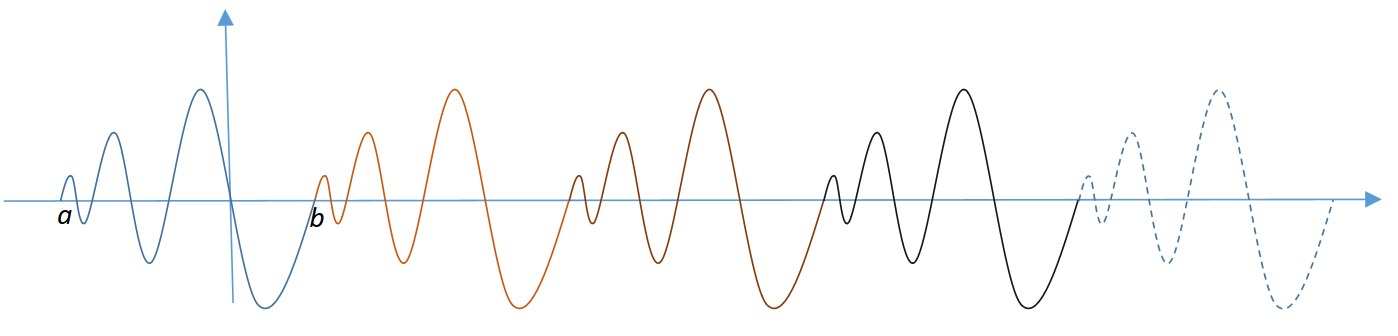
\includegraphics{images/signals_aperiodic.png}
   \caption{Repeating an aperiodic signal results in a periodic one}
   \label{fig:signals_aperiodic}
\end{figure}


\subsection{Combining and decomposing signals}
It is possible to combine signals, e.g. by adding them together, to create new signals.
\begin{figure}[htbp]
   \centering
   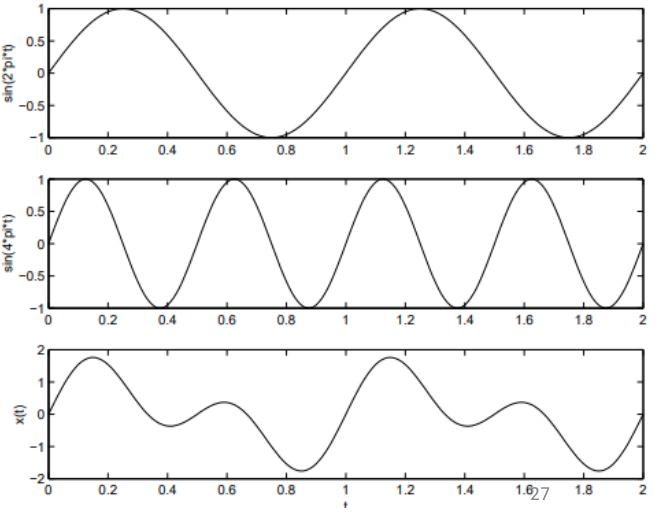
\includegraphics{images/signals_combination.png}
   \label{fig:signals_combination}

   $x_t = \sin(2\pi t) + \sin(4\pi t)$
\end{figure}

The Fourier series allows to decompose a periodic signal into a sum of sines and cosines, inverting the combining process.
More formally the Fourier series\ul{ decomposes a function (signal) as the sum of an infinite number of continuous functions, oscillating at
different frequencies.}\\
This set of continuous functions defines the base of
decomposition.
The Fourier series has a base represented by a set of functions
\[
   \phi_n(t) , n \in \mathbb{Z}
\]
This set of functions must be orthogonal (as in the case of decomposition of vectors in a vector space)
\newpage
\begin{definition}[Fourier series]
   Given a continuous signal $s(t) : \mathbb{R} \rightarrow \mathbb{R}$, periodic in the interval $[-\pi, \pi]$ its Fourier
   series is defined as:
   \begin{figure}[htbp]
      \centering
      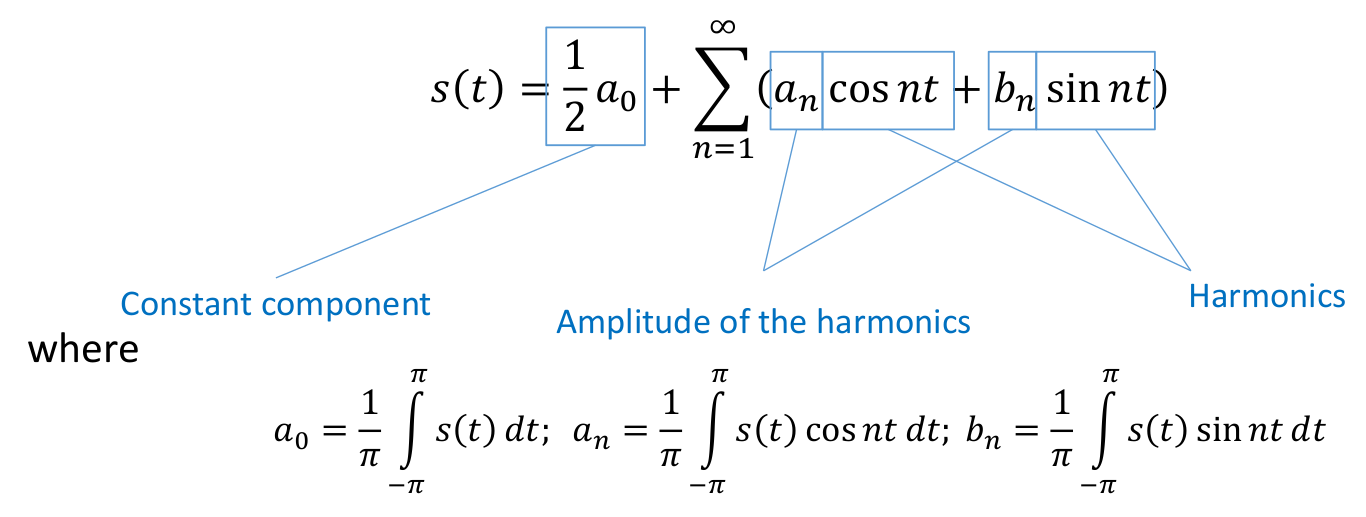
\includegraphics{images/fourierseries.png}
      % \caption{Fourier series}
      \label{fig:fourierseries}
   \end{figure}
\end{definition}

It is rather complicate to assess the conditions under which an arbitrary $s(t)$ can be developed in a Fourier series, in particular necessary conditions are \textit{not} known; however, there are sufficient conditions:
\begin{theorem}[Dirichlet]
   
   \nl
   \begin{enumerate}
      \item $s(t)$ is periodic
      \item $s(t)$ is piecewise continuous
      \item[$\Rightarrow$] the Fourier series of $s(t)$ exists and converges in $\mathbb{R}$
   \end{enumerate}
   \end{theorem}
A \textit{piecewise continuous} function is made up of a finite number of continuous pieces on each finite subinterval $[0,T]$. Also the
limit of $f(t)$ as $t$ tends to each point of discontinuity is finite.

\section{Energy and Power signals}
\begin{definition}[Energy]
   The \textbf{energy} $E$ of a signal $s(t)$ is given by:
   \begin{equation}
      E(T) \stackrel{\triangle}{=} \int_{-\frac{T}{2}}^{+\frac{T}{2}} |s(t)|^2 dt
   \end{equation}
\end{definition}

The signal has \textit{finite energy} (is an \textbf{energy signal}) if the limit of $E(T)$ as $T$ tends to infinity is finite:

\begin{align}
0 & < & \lim_{T \to \infty} E(T) &< & +\infty\\
0 & < & E_s = \int_{-\infty}^{+\infty} |s(t)|^2 dt &< & +\infty
\end{align}

Even infinite signals may have finite energy. In the physical world, all signals have finite energy.

\nl

\begin{definition}[Power]
   The \textbf{power} $P_f$ of a signal $s(t)$ is given by:
   \begin{equation}
   P_f(T) \stackrel{\triangle}{=} \frac{1}{T} \int_{-\frac{T}{2}}^{+\frac{T}{2}} |s(t)|^2 dt = \frac{E_s(T)}{T}
   \end{equation}
\end{definition}

The signal has \textit{finite power} (is a \textbf{power signal}) if the limit of $P(T)$ as $T$ tends to infinity is finite:

\begin{align}
   0 & < & P_s = \lim_{T \to \infty} \frac{1}{T} \int_{-\frac{T}{2}}^{+\frac{T}{2}} |s(t)|^2 dt & < & +\infty
\end{align}

\textbf{Periodic signals} have some peculiarities in terms of power and energy:
\begin{itemize}
   \item They have infinite energy
   \begin{itemize}
      \item They are \textit{power signals}, \ul{not} energy signals
   \end{itemize}
   \item Their average power equals the average power computed in a single period 
\end{itemize} 

\begin{figure}[htbp]
   \centering
   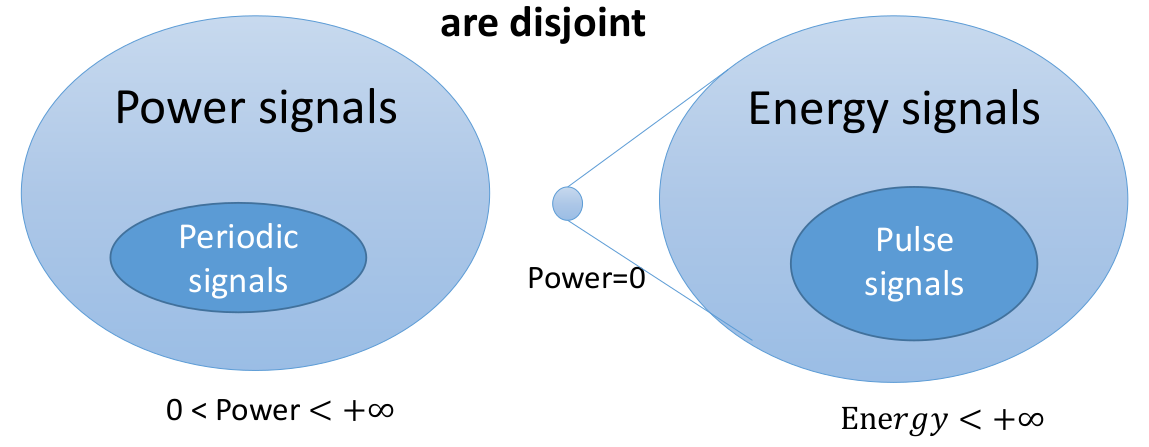
\includegraphics{images/powerenergy_signals.png}
   \caption{Power and energy signals classes}
   \begin{enumerate}
      \item 
      A signal may be an energy signal, a power signal, or none
      \item A signal cannot be both an energy signal and a power signal
   \end{enumerate}
      \label{fig:powerenergy_signals}
\end{figure}

\section{Fourier Transform}
\subsection{Preliminaries}
\begin{definition}[Complex numbers]
   A complex number $\bar{x}$ is a number of the form $x = a + jb$, where $a$ and $b$ are real numbers and $j$ is the imaginary unit, the square root of $-1$.

   It may be represented in the imaginary plane as a vector with modulus $|x| = \sqrt{a^2 + b^2}$ and phase $\Phi$

   \begin{figure}[htbp]
      \centering
      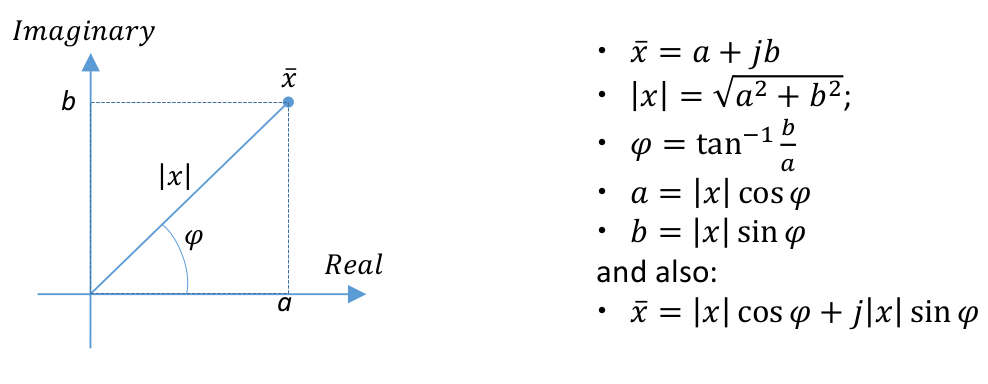
\includegraphics{images/complex_vector.png}
      \caption{Complex number in the imaginary plane}
      \label{fig:complex_vector}
   \end{figure}
\end{definition}

\begin{definition}
   [Euler's exponential]
   The exponential $e^{j\theta}$ is a complex number that can be represented in the imaginary plane as a vector of modulus 1 and phase $\theta$. It is defined as:
   \begin{equation}
      e^{j\theta} = \cos(\theta) + j\sin(\theta)
   \end{equation}
   From which we can derive Euler's formulas:
   \begin{align}
      \cos(\theta) & = \frac{e^{j\theta} + e^{-j\theta}}{2}\\
      \sin(\theta) & = \frac{e^{j\theta} - e^{-j\theta}}{2j}
   \end{align}
\end{definition}

A complex number may also be written as $x = |x|e^{j\Phi}$, where $|x|$ is the modulus and $\Phi$ is the phase.
The conjugate of $\bar{x}$ may also be written as $\bar{x} = |x|e^{-j\Phi}$

The Fourier series is usually expressed in the complex number domain, to represent signals $s(t): \mathbb{R} \rightarrow \mathbb{C}$

The \textbf{base of Fourier} is the set of functions:
\begin{equation}
   % \phi_n(t) = e^{j\frac{2\pi n}{T}t}
   e^{j2\pi n F t} \forall n \in \mathbb{Z}
\end{equation}
Considering also the definition of the exponential $e^{x + jy}$, we get the last equation:
\begin{align}
   e^{x + jy} & = & e^x e^{jy} =e^x(\cos(y) + j\sin(y))\\
   e^{j2\pi n F t} & = & \cos(2\pi n F t) + j\sin(2\pi n F t)
\end{align}
\nl


\newpage
\begin{definition}
   [Fourier series with exponential base]
   Given a periodic signal $s(t)$ with frequency $F = 1/T$, we can represent it as a linear combination
   \begin{equation}
      s(t) = \sum_{n=-\infty}^{+\infty} S_n e^{j2\pi n F t}
   \end{equation} 
   Where $S_n$ is the ---Fourier--- series:
   \begin{equation}
      S_n = \frac{1}{T} \int_0^T s(t) e^{-j2\pi n F t} dt
   \end{equation}
\end{definition}

\begin{figure}[htbp]
   \centering
   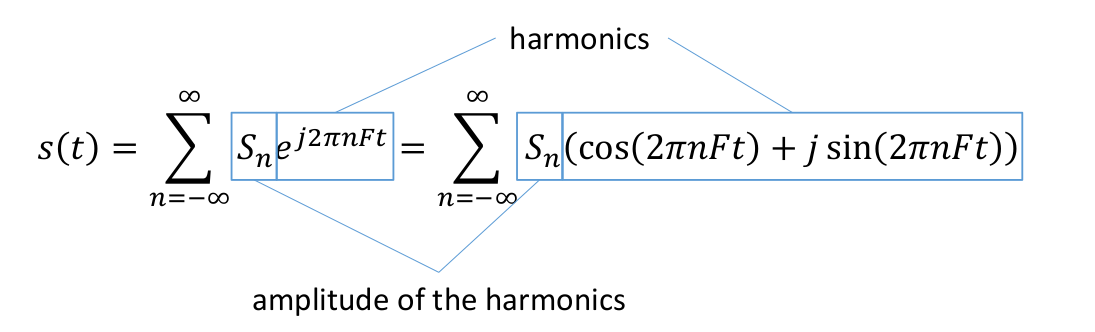
\includegraphics{images/fourier_geometric.png}
   \caption{Fourier Geometrical interpretation}
   \label{fig:fourier_geometric}
\end{figure}

\begin{definition}
   [Signal Spectrum]
   The \textbf{spectrum} of a signal is the ordered set of its Fourier coefficients $S_n$ from $n = -\infty$ to $n = +\infty$.
   \note{The spectrum may be seen as a discrete signal}
\end{definition}

\begin{definition}
   [Fourier Transform]
   The transition from the continuous signal $s(t)$ to its spectrum i.e. to its discrete signal $S_n$ is called the \textbf{Fourier Transform}, denoted in the following ways

   \begin{align}
      s(t) & \xLeftrightarrow{\text{FT}} S_n\\
      S_n & = \mathcal{F}(s(t)) & \textit{transform}\\
      s(t) & = \mathcal{F}^{-1}(S_n) & \textit{inverse transform}
   \end{align}
\end{definition}

$S_n$ may be also represented using the Euler's exponential, with the first term being the \textit{amplitude} of the harmonics, and the $e$ the \textit{phase} of harmonics:
\begin{equation}
   S_n=|S_n|e^{j\theta_n}
\end{equation}

\section{From FT to Discrete FT}
\note{Non ho capito molto di questa cosa}
In the field of digital signal processing, signals and spectra are processed only in sampled form.
\begin{itemize}
   \item We have a signal s known only at a finite number instants separated by sample times (i.e. a finite sequence of data)
   \item We want to compute a finite number of samples of the Fourier Transform so that\dots
   \item Discrete-time data sets are converted into a finite discrete-frequency representation
\end{itemize}

Discrete time signals are typically obtained from continuous signals with a domain restriction from $\mathbb{R}$ into $\mathbb{Z}(T)$.
This operation, called \textbf{sampling}, is stated by the simple relationship
\(
   sc(nT) = s(nT) , nT \in \mathbb{Z}(T)
\)
Where $s(t) , t \in \mathbb{R}$, is the reference continuous signal, while $s(nT)$ is the corresponding sampled discrete signal.

\begin{definition}
   [Discrete signal]
   A discrete signal is a complex function of a discrete variable:
   \[
      f(t)= \mathbb{Z}(T) \rightarrow \mathcal{C}
   \]
   Where $\mathbb{Z}(T)$ is the subset of $\mathbb{Z}$ made up only of $T>0$ multiples ${\dots -T,0,T,2T}$
\end{definition}

\note{TODO altre equazioni complicate}